\section{Twisted Metal: }

\begin{figure}[htbp]
\begin{center}
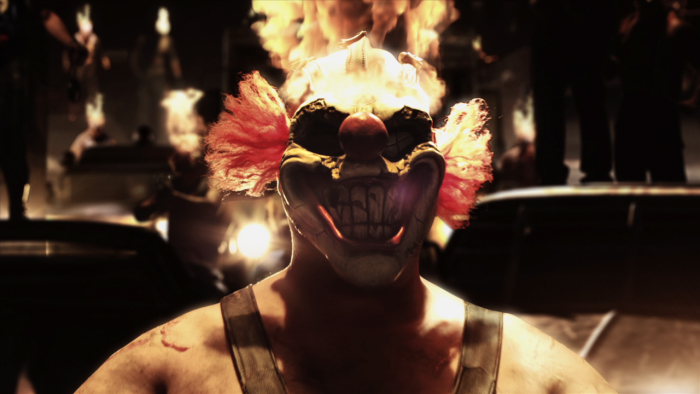
\includegraphics[width=.60\textwidth]{./imagenes/twistedmetal.jpg}
\caption{Twisted Metal}
\end{center}
\end{figure}

Twisted Metal es la primera entrega de la serie Twisted Metal. La historia del juego está centrada en el titular de la competencia en la que varios conductores de vehículos modificados deben destruir los otros vehículos en un intento por ser el último vivo. El ganador se reúne con el organizador de la competición, un misterioso hombre llamado Calypso, que otorgará al ganador un único deseo, independientemente de su precio, tamaño, o incluso de la realidad.
Twisted Metal recibió críticas dispares de la prensa especializada, pero el juego fue un éxito comercial, vendiendo más de 1.800.000 copias en los Estados Unidos.
\subsubsection{¿Por qué es uno de mis juegos favoritos?}
\begin{itemize}
\item[Juan Romero ] Twisted Metal es una de mis franquicias de juegos favoritos. He sido  fan desde hace mucho tiempo y comenzé a jugar la serie con Twisted Metal 3 para la consola de PlayStation 1 . Lo que me gustó de la experiencia fue que se combinan de forma única los juegos de conducción con los de  shooter en primera persona. Matar a los oponentes y ver como volaban en mil pedasos era lo que mas me divertia, ademas el hecho de que habia que tener buenas habilidades para manejar un vehículo,matar y estar pendiente de eludir los ataques de los demas contrincantes.
\end{itemize}